% VDE Template for EUSAR Papers
% Provided by Barbara Lang und Siegmar Lampe
% University of Bremen, January 2002
% English version by Jens Fischer
% German Aerospace Center (DLR), December 2005
% Additional modifications by Matthias Wei{\ss}
% FGAN, January 2009

%-----------------------------------------------------------------------------
% Type of publication
\documentclass[a4paper,10pt]{article}
%-----------------------------------------------------------------------------
% Other packets: Most packets may be downloaded from www.dante.de and
% "tcilatex.tex" can be found at (December 2005):
% http://www.mackichan.com/techtalk/v30/UsingFloat.htm
% Not all packets are necessarily needed:
\usepackage[T1]{fontenc}
\usepackage[latin1]{inputenc}
%\usepackage{ngerman} % in german language if required
\usepackage[nooneline,bf,scriptsize]{caption} % Figure descriptions from left margin
\usepackage{times}
\usepackage{multicol}
\usepackage{tabularx}
\usepackage{booktabs}
\usepackage{amsmath}
\usepackage{amssymb}
\usepackage[dvips]{graphicx}
\usepackage{epsfig}
\usepackage{listings}
\usepackage[titletoc,toc,title]{appendix}
\usepackage[breaklinks]{hyperref}
\usepackage{url}
\def\Urlbreaks{\do\/\do-}
\usepackage{breakurl}
% Macros for Scientific Word 3.0 documents saved with the LaTeX filter.
%Copyright (C) 1994-97 TCI Software Research, Inc.
\typeout{TCILATEX Macros for Scientific Word 3.0 <05 August 1998>.}
\typeout{NOTICE:  This macro file is NOT proprietary and may be 
freely copied and distributed.}
%
\makeatletter
%
%%%%%%%%%%%%%%%%%%%%%%
% macros for time
\newcount\@hour\newcount\@minute\chardef\@x10\chardef\@xv60
\def\tcitime{
\def\@time{%
  \@minute\time\@hour\@minute\divide\@hour\@xv
  \ifnum\@hour<\@x 0\fi\the\@hour:%
  \multiply\@hour\@xv\advance\@minute-\@hour
  \ifnum\@minute<\@x 0\fi\the\@minute
  }}%

%%%%%%%%%%%%%%%%%%%%%%
% macro for hyperref
\@ifundefined{hyperref}{\def\hyperref#1#2#3#4{#2\ref{#4}#3}}{}

% macro for external program call
\@ifundefined{qExtProgCall}{\def\qExtProgCall#1#2#3#4#5#6{\relax}}{}
%%%%%%%%%%%%%%%%%%%%%%
%
% macros for graphics
%
\def\FILENAME#1{#1}%
%
\def\QCTOpt[#1]#2{%
  \def\QCTOptB{#1}
  \def\QCTOptA{#2}
}
\def\QCTNOpt#1{%
  \def\QCTOptA{#1}
  \let\QCTOptB\empty
}
\def\Qct{%
  \@ifnextchar[{%
    \QCTOpt}{\QCTNOpt}
}
\def\QCBOpt[#1]#2{%
  \def\QCBOptB{#1}
  \def\QCBOptA{#2}
}
\def\QCBNOpt#1{%
  \def\QCBOptA{#1}
  \let\QCBOptB\empty
}
\def\Qcb{%
  \@ifnextchar[{%
    \QCBOpt}{\QCBNOpt}
}
\def\PrepCapArgs{%
  \ifx\QCBOptA\empty
    \ifx\QCTOptA\empty
      {}%
    \else
      \ifx\QCTOptB\empty
        {\QCTOptA}%
      \else
        [\QCTOptB]{\QCTOptA}%
      \fi
    \fi
  \else
    \ifx\QCBOptA\empty
      {}%
    \else
      \ifx\QCBOptB\empty
        {\QCBOptA}%
      \else
        [\QCBOptB]{\QCBOptA}%
      \fi
    \fi
  \fi
}
\newcount\GRAPHICSTYPE
%\GRAPHICSTYPE 0 is for TurboTeX
%\GRAPHICSTYPE 1 is for DVIWindo (PostScript)
%%%(removed)%\GRAPHICSTYPE 2 is for psfig (PostScript)
\GRAPHICSTYPE=\z@
\def\GRAPHICSPS#1{%
 \ifcase\GRAPHICSTYPE%\GRAPHICSTYPE=0
   \special{ps: #1}%
 \or%\GRAPHICSTYPE=1
   \special{language "PS", include "#1"}%
%%%\or%\GRAPHICSTYPE=2
%%%  #1%
 \fi
}%
%
\def\GRAPHICSHP#1{\special{include #1}}%
%
% \graffile{ body }                                  %#1
%          { contentswidth (scalar)  }               %#2
%          { contentsheight (scalar) }               %#3
%          { vertical shift when in-line (scalar) }  %#4
\def\graffile#1#2#3#4{%
%%% \ifnum\GRAPHICSTYPE=\tw@
%%%  %Following if using psfig
%%%  \@ifundefined{psfig}{\input psfig.tex}{}%
%%%  \psfig{file=#1, height=#3, width=#2}%
%%% \else
  %Following for all others
  % JCS - added BOXTHEFRAME, see below
    \bgroup
    \leavevmode
    \@ifundefined{bbl@deactivate}{\def~{\string~}}{\activesoff}
    \raise -#4 \BOXTHEFRAME{%
        \hbox to #2{\raise #3\hbox to #2{\null #1\hfil}}}%
    \egroup
}%
%
% A box for drafts
\def\draftbox#1#2#3#4{%
 \leavevmode\raise -#4 \hbox{%
  \frame{\rlap{\protect\tiny #1}\hbox to #2%
   {\vrule height#3 width\z@ depth\z@\hfil}%
  }%
 }%
}%
%
\newcount\draft
\draft=\z@
\let\nographics=\draft
\newif\ifwasdraft
\wasdraftfalse

%  \GRAPHIC{ body }                                  %#1
%          { draft name }                            %#2
%          { contentswidth (scalar)  }               %#3
%          { contentsheight (scalar) }               %#4
%          { vertical shift when in-line (scalar) }  %#5
\def\GRAPHIC#1#2#3#4#5{%
 \ifnum\draft=\@ne\draftbox{#2}{#3}{#4}{#5}%
  \else\graffile{#1}{#3}{#4}{#5}%
  \fi
 }%
%
\def\addtoLaTeXparams#1{%
    \edef\LaTeXparams{\LaTeXparams #1}}%
%
% JCS -  added a switch BoxFrame that can 
% be set by including X in the frame params.
% If set a box is drawn around the frame.

\newif\ifBoxFrame \BoxFramefalse
\newif\ifOverFrame \OverFramefalse
\newif\ifUnderFrame \UnderFramefalse

\def\BOXTHEFRAME#1{%
   \hbox{%
      \ifBoxFrame
         \frame{#1}%
      \else
         {#1}%
      \fi
   }%
}


\def\doFRAMEparams#1{\BoxFramefalse\OverFramefalse\UnderFramefalse\readFRAMEparams#1\end}%
\def\readFRAMEparams#1{%
 \ifx#1\end%
  \let\next=\relax
  \else
  \ifx#1i\dispkind=\z@\fi
  \ifx#1d\dispkind=\@ne\fi
  \ifx#1f\dispkind=\tw@\fi
  \ifx#1t\addtoLaTeXparams{t}\fi
  \ifx#1b\addtoLaTeXparams{b}\fi
  \ifx#1p\addtoLaTeXparams{p}\fi
  \ifx#1h\addtoLaTeXparams{h}\fi
  \ifx#1X\BoxFrametrue\fi
  \ifx#1O\OverFrametrue\fi
  \ifx#1U\UnderFrametrue\fi
  \ifx#1w
    \ifnum\draft=1\wasdrafttrue\else\wasdraftfalse\fi
    \draft=\@ne
  \fi
  \let\next=\readFRAMEparams
  \fi
 \next
 }%
%
%Macro for In-line graphics object
%   \IFRAME{ contentswidth (scalar)  }               %#1
%          { contentsheight (scalar) }               %#2
%          { vertical shift when in-line (scalar) }  %#3
%          { draft name }                            %#4
%          { body }                                  %#5
%          { caption}                                %#6


\def\IFRAME#1#2#3#4#5#6{%
      \bgroup
      \let\QCTOptA\empty
      \let\QCTOptB\empty
      \let\QCBOptA\empty
      \let\QCBOptB\empty
      #6%
      \parindent=0pt%
      \leftskip=0pt
      \rightskip=0pt
      \setbox0 = \hbox{\QCBOptA}%
      \@tempdima = #1\relax
      \ifOverFrame
          % Do this later
          \typeout{This is not implemented yet}%
          \show\HELP
      \else
         \ifdim\wd0>\@tempdima
            \advance\@tempdima by \@tempdima
            \ifdim\wd0 >\@tempdima
               \textwidth=\@tempdima
               \setbox1 =\vbox{%
                  \noindent\hbox to \@tempdima{\hfill\GRAPHIC{#5}{#4}{#1}{#2}{#3}\hfill}\\%
                  \noindent\hbox to \@tempdima{\parbox[b]{\@tempdima}{\QCBOptA}}%
               }%
               \wd1=\@tempdima
            \else
               \textwidth=\wd0
               \setbox1 =\vbox{%
                 \noindent\hbox to \wd0{\hfill\GRAPHIC{#5}{#4}{#1}{#2}{#3}\hfill}\\%
                 \noindent\hbox{\QCBOptA}%
               }%
               \wd1=\wd0
            \fi
         \else
            %\show\BBB
            \ifdim\wd0>0pt
              \hsize=\@tempdima
              \setbox1 =\vbox{%
                \unskip\GRAPHIC{#5}{#4}{#1}{#2}{0pt}%
                \break
                \unskip\hbox to \@tempdima{\hfill \QCBOptA\hfill}%
              }%
              \wd1=\@tempdima
           \else
              \hsize=\@tempdima
              \setbox1 =\vbox{%
                \unskip\GRAPHIC{#5}{#4}{#1}{#2}{0pt}%
              }%
              \wd1=\@tempdima
           \fi
         \fi
         \@tempdimb=\ht1
         \advance\@tempdimb by \dp1
         \advance\@tempdimb by -#2%
         \advance\@tempdimb by #3%
         \leavevmode
         \raise -\@tempdimb \hbox{\box1}%
      \fi
      \egroup%
}%
%
%Macro for Display graphics object
%   \DFRAME{ contentswidth (scalar)  }               %#1
%          { contentsheight (scalar) }               %#2
%          { draft label }                           %#3
%          { name }                                  %#4
%          { caption}                                %#5
\def\DFRAME#1#2#3#4#5{%
 \begin{center}
     \let\QCTOptA\empty
     \let\QCTOptB\empty
     \let\QCBOptA\empty
     \let\QCBOptB\empty
     \ifOverFrame 
        #5\QCTOptA\par
     \fi
     \GRAPHIC{#4}{#3}{#1}{#2}{\z@}
     \ifUnderFrame 
        \nobreak\par\nobreak#5\QCBOptA
     \fi
 \end{center}%
 }%
%
%Macro for Floating graphic object
%   \FFRAME{ framedata f|i tbph x F|T }              %#1
%          { contentswidth (scalar)  }               %#2
%          { contentsheight (scalar) }               %#3
%          { caption }                               %#4
%          { label }                                 %#5
%          { draft name }                            %#6
%          { body }                                  %#7
\def\FFRAME#1#2#3#4#5#6#7{%
 %If float.sty loaded and float option is 'h', change to 'H'  (gp) 1998/09/05
  \@ifundefined{floatstyle}
    {%floatstyle undefined (and float.sty not present), no change
     \begin{figure}[#1]%
    }
    {%floatstyle DEFINED
	 \ifx#1h%Only the h parameter, change to H
      \begin{figure}[H]%
	 \else
      \begin{figure}[#1]%
	 \fi
	}
  \let\QCTOptA\empty
  \let\QCTOptB\empty
  \let\QCBOptA\empty
  \let\QCBOptB\empty
  \ifOverFrame
    #4
    \ifx\QCTOptA\empty
    \else
      \ifx\QCTOptB\empty
        \caption{\QCTOptA}%
      \else
        \caption[\QCTOptB]{\QCTOptA}%
      \fi
    \fi
    \ifUnderFrame\else
      \label{#5}%
    \fi
  \else
    \UnderFrametrue%
  \fi
  \begin{center}\GRAPHIC{#7}{#6}{#2}{#3}{\z@}\end{center}%
  \ifUnderFrame
    #4
    \ifx\QCBOptA\empty
      \caption{}%
    \else
      \ifx\QCBOptB\empty
        \caption{\QCBOptA}%
      \else
        \caption[\QCBOptB]{\QCBOptA}%
      \fi
    \fi
    \label{#5}%
  \fi
  \end{figure}%
 }%
%
%
%    \FRAME{ framedata f|i tbph x F|T }              %#1
%          { contentswidth (scalar)  }               %#2
%          { contentsheight (scalar) }               %#3
%          { vertical shift when in-line (scalar) }  %#4
%          { caption }                               %#5
%          { label }                                 %#6
%          { name }                                  %#7
%          { body }                                  %#8
%
%    framedata is a string which can contain the following
%    characters: idftbphxFT
%    Their meaning is as follows:
%             i, d or f : in-line, display, or floating
%             t,b,p,h   : LaTeX floating placement options
%             x         : fit contents box to contents
%             F or T    : Figure or Table. 
%                         Later this can expand
%                         to a more general float class.
%
%
\newcount\dispkind%

\def\makeactives{
  \catcode`\"=\active
  \catcode`\;=\active
  \catcode`\:=\active
  \catcode`\'=\active
  \catcode`\~=\active
}
\bgroup
   \makeactives
   \gdef\activesoff{%
      \def"{\string"}
      \def;{\string;}
      \def:{\string:}
      \def'{\string'}
      \def~{\string~}
      %\bbl@deactivate{"}%
      %\bbl@deactivate{;}%
      %\bbl@deactivate{:}%
      %\bbl@deactivate{'}%
    }
\egroup

\def\FRAME#1#2#3#4#5#6#7#8{%
 \bgroup
 \ifnum\draft=\@ne
   \wasdrafttrue
 \else
   \wasdraftfalse%
 \fi
 \def\LaTeXparams{}%
 \dispkind=\z@
 \def\LaTeXparams{}%
 \doFRAMEparams{#1}%
 \ifnum\dispkind=\z@\IFRAME{#2}{#3}{#4}{#7}{#8}{#5}\else
  \ifnum\dispkind=\@ne\DFRAME{#2}{#3}{#7}{#8}{#5}\else
   \ifnum\dispkind=\tw@
    \edef\@tempa{\noexpand\FFRAME{\LaTeXparams}}%
    \@tempa{#2}{#3}{#5}{#6}{#7}{#8}%
    \fi
   \fi
  \fi
  \ifwasdraft\draft=1\else\draft=0\fi{}%
  \egroup
 }%
%
% This macro added to let SW gobble a parameter that
% should not be passed on and expanded. 

\def\TEXUX#1{"texux"}

%
% Macros for text attributes:
%
\def\BF#1{{\bf {#1}}}%
\def\NEG#1{\leavevmode\hbox{\rlap{\thinspace/}{$#1$}}}%
%
%%%%%%%%%%%%%%%%%%%%%%%%%%%%%%%%%%%%%%%%%%%%%%%%%%%%%%%%%%%%%%%%%%%%%%%%
%
%
% macros for user - defined functions
\def\limfunc#1{\mathop{\rm #1}}%
\def\func#1{\mathop{\rm #1}\nolimits}%
% macro for unit names
\def\unit#1{\mathop{\rm #1}\nolimits}%

%
% miscellaneous 
\long\def\QQQ#1#2{%
     \long\expandafter\def\csname#1\endcsname{#2}}%
\@ifundefined{QTP}{\def\QTP#1{}}{}
\@ifundefined{QEXCLUDE}{\def\QEXCLUDE#1{}}{}
\@ifundefined{Qlb}{\def\Qlb#1{#1}}{}
\@ifundefined{Qlt}{\def\Qlt#1{#1}}{}
\def\QWE{}%
\long\def\QQA#1#2{}%
\def\QTR#1#2{{\csname#1\endcsname #2}}%(gp) Is this the best?
\long\def\TeXButton#1#2{#2}%
\long\def\QSubDoc#1#2{#2}%
\def\EXPAND#1[#2]#3{}%
\def\NOEXPAND#1[#2]#3{}%
\def\PROTECTED{}%
\def\LaTeXparent#1{}%
\def\ChildStyles#1{}%
\def\ChildDefaults#1{}%
\def\QTagDef#1#2#3{}%

% Constructs added with Scientific Notebook
\@ifundefined{correctchoice}{\def\correctchoice{\relax}}{}
\@ifundefined{HTML}{\def\HTML#1{\relax}}{}
\@ifundefined{TCIIcon}{\def\TCIIcon#1#2#3#4{\relax}}{}
\if@compatibility
  \typeout{Not defining UNICODE or CustomNote commands for LaTeX 2.09.}
\else
  \providecommand{\UNICODE}[2][]{}
  \providecommand{\CustomNote}[3][]{\marginpar{#3}}
\fi

%
% Macros for style editor docs
\@ifundefined{StyleEditBeginDoc}{\def\StyleEditBeginDoc{\relax}}{}
%
% Macros for footnotes
\def\QQfnmark#1{\footnotemark}
\def\QQfntext#1#2{\addtocounter{footnote}{#1}\footnotetext{#2}}
%
% Macros for indexing.
%
\@ifundefined{TCIMAKEINDEX}{}{\makeindex}%
%
% Attempts to avoid problems with other styles
\@ifundefined{abstract}{%
 \def\abstract{%
  \if@twocolumn
   \section*{Abstract (Not appropriate in this style!)}%
   \else \small 
   \begin{center}{\bf Abstract\vspace{-.5em}\vspace{\z@}}\end{center}%
   \quotation 
   \fi
  }%
 }{%
 }%
\@ifundefined{endabstract}{\def\endabstract
  {\if@twocolumn\else\endquotation\fi}}{}%
\@ifundefined{maketitle}{\def\maketitle#1{}}{}%
\@ifundefined{affiliation}{\def\affiliation#1{}}{}%
\@ifundefined{proof}{\def\proof{\noindent{\bfseries Proof. }}}{}%
\@ifundefined{endproof}{\def\endproof{\mbox{\ \rule{.1in}{.1in}}}}{}%
\@ifundefined{newfield}{\def\newfield#1#2{}}{}%
\@ifundefined{chapter}{\def\chapter#1{\par(Chapter head:)#1\par }%
 \newcount\c@chapter}{}%
\@ifundefined{part}{\def\part#1{\par(Part head:)#1\par }}{}%
\@ifundefined{section}{\def\section#1{\par(Section head:)#1\par }}{}%
\@ifundefined{subsection}{\def\subsection#1%
 {\par(Subsection head:)#1\par }}{}%
\@ifundefined{subsubsection}{\def\subsubsection#1%
 {\par(Subsubsection head:)#1\par }}{}%
\@ifundefined{paragraph}{\def\paragraph#1%
 {\par(Subsubsubsection head:)#1\par }}{}%
\@ifundefined{subparagraph}{\def\subparagraph#1%
 {\par(Subsubsubsubsection head:)#1\par }}{}%
%%%%%%%%%%%%%%%%%%%%%%%%%%%%%%%%%%%%%%%%%%%%%%%%%%%%%%%%%%%%%%%%%%%%%%%%
% These symbols are not recognized by LaTeX
\@ifundefined{therefore}{\def\therefore{}}{}%
\@ifundefined{backepsilon}{\def\backepsilon{}}{}%
\@ifundefined{yen}{\def\yen{\hbox{\rm\rlap=Y}}}{}%
\@ifundefined{registered}{%
   \def\registered{\relax\ifmmode{}\r@gistered
                    \else$\m@th\r@gistered$\fi}%
 \def\r@gistered{^{\ooalign
  {\hfil\raise.07ex\hbox{$\scriptstyle\rm\text{R}$}\hfil\crcr
  \mathhexbox20D}}}}{}%
\@ifundefined{Eth}{\def\Eth{}}{}%
\@ifundefined{eth}{\def\eth{}}{}%
\@ifundefined{Thorn}{\def\Thorn{}}{}%
\@ifundefined{thorn}{\def\thorn{}}{}%
% A macro to allow any symbol that requires math to appear in text
\def\TEXTsymbol#1{\mbox{$#1$}}%
\@ifundefined{degree}{\def\degree{{}^{\circ}}}{}%
%
% macros for T3TeX files
\newdimen\theight
\def\Column{%
 \vadjust{\setbox\z@=\hbox{\scriptsize\quad\quad tcol}%
  \theight=\ht\z@\advance\theight by \dp\z@\advance\theight by \lineskip
  \kern -\theight \vbox to \theight{%
   \rightline{\rlap{\box\z@}}%
   \vss
   }%
  }%
 }%
%
\def\qed{%
 \ifhmode\unskip\nobreak\fi\ifmmode\ifinner\else\hskip5\p@\fi\fi
 \hbox{\hskip5\p@\vrule width4\p@ height6\p@ depth1.5\p@\hskip\p@}%
 }%
%
\def\cents{\hbox{\rm\rlap/c}}%
\def\miss{\hbox{\vrule height2\p@ width 2\p@ depth\z@}}%
%
\def\vvert{\Vert}%           %always translated to \left| or \right|
%
\def\tcol#1{{\baselineskip=6\p@ \vcenter{#1}} \Column}  %
%
\def\dB{\hbox{{}}}%                 %dummy entry in column 
\def\mB#1{\hbox{$#1$}}%             %column entry
\def\nB#1{\hbox{#1}}%               %column entry (not math)
%
\@ifundefined{note}{\def\note{$^{\dag}}}{}%
%

\def\newfmtname{LaTeX2e}
% No longer load latexsym.  This is now handled by SWP, which uses amsfonts if necessary

\ifx\fmtname\newfmtname
  \DeclareOldFontCommand{\rm}{\normalfont\rmfamily}{\mathrm}
  \DeclareOldFontCommand{\sf}{\normalfont\sffamily}{\mathsf}
  \DeclareOldFontCommand{\tt}{\normalfont\ttfamily}{\mathtt}
  \DeclareOldFontCommand{\bf}{\normalfont\bfseries}{\mathbf}
  \DeclareOldFontCommand{\it}{\normalfont\itshape}{\mathit}
  \DeclareOldFontCommand{\sl}{\normalfont\slshape}{\@nomath\sl}
  \DeclareOldFontCommand{\sc}{\normalfont\scshape}{\@nomath\sc}
\fi

%
% Greek bold macros
% Redefine all of the math symbols 
% which might be bolded	 - there are 
% probably others to add to this list

\def\alpha{{\Greekmath 010B}}%
\def\beta{{\Greekmath 010C}}%
\def\gamma{{\Greekmath 010D}}%
\def\delta{{\Greekmath 010E}}%
\def\epsilon{{\Greekmath 010F}}%
\def\zeta{{\Greekmath 0110}}%
\def\eta{{\Greekmath 0111}}%
\def\theta{{\Greekmath 0112}}%
\def\iota{{\Greekmath 0113}}%
\def\kappa{{\Greekmath 0114}}%
\def\lambda{{\Greekmath 0115}}%
\def\mu{{\Greekmath 0116}}%
\def\nu{{\Greekmath 0117}}%
\def\xi{{\Greekmath 0118}}%
\def\pi{{\Greekmath 0119}}%
\def\rho{{\Greekmath 011A}}%
\def\sigma{{\Greekmath 011B}}%
\def\tau{{\Greekmath 011C}}%
\def\upsilon{{\Greekmath 011D}}%
\def\phi{{\Greekmath 011E}}%
\def\chi{{\Greekmath 011F}}%
\def\psi{{\Greekmath 0120}}%
\def\omega{{\Greekmath 0121}}%
\def\varepsilon{{\Greekmath 0122}}%
\def\vartheta{{\Greekmath 0123}}%
\def\varpi{{\Greekmath 0124}}%
\def\varrho{{\Greekmath 0125}}%
\def\varsigma{{\Greekmath 0126}}%
\def\varphi{{\Greekmath 0127}}%

\def\nabla{{\Greekmath 0272}}
\def\FindBoldGroup{%
   {\setbox0=\hbox{$\mathbf{x\global\edef\theboldgroup{\the\mathgroup}}$}}%
}

\def\Greekmath#1#2#3#4{%
    \if@compatibility
        \ifnum\mathgroup=\symbold
           \mathchoice{\mbox{\boldmath$\displaystyle\mathchar"#1#2#3#4$}}%
                      {\mbox{\boldmath$\textstyle\mathchar"#1#2#3#4$}}%
                      {\mbox{\boldmath$\scriptstyle\mathchar"#1#2#3#4$}}%
                      {\mbox{\boldmath$\scriptscriptstyle\mathchar"#1#2#3#4$}}%
        \else
           \mathchar"#1#2#3#4% 
        \fi 
    \else 
        \FindBoldGroup
        \ifnum\mathgroup=\theboldgroup % For 2e
           \mathchoice{\mbox{\boldmath$\displaystyle\mathchar"#1#2#3#4$}}%
                      {\mbox{\boldmath$\textstyle\mathchar"#1#2#3#4$}}%
                      {\mbox{\boldmath$\scriptstyle\mathchar"#1#2#3#4$}}%
                      {\mbox{\boldmath$\scriptscriptstyle\mathchar"#1#2#3#4$}}%
        \else
           \mathchar"#1#2#3#4% 
        \fi     	    
	  \fi}

\newif\ifGreekBold  \GreekBoldfalse
\let\SAVEPBF=\pbf
\def\pbf{\GreekBoldtrue\SAVEPBF}%
%

\@ifundefined{theorem}{\newtheorem{theorem}{Theorem}}{}
\@ifundefined{lemma}{\newtheorem{lemma}[theorem]{Lemma}}{}
\@ifundefined{corollary}{\newtheorem{corollary}[theorem]{Corollary}}{}
\@ifundefined{conjecture}{\newtheorem{conjecture}[theorem]{Conjecture}}{}
\@ifundefined{proposition}{\newtheorem{proposition}[theorem]{Proposition}}{}
\@ifundefined{axiom}{\newtheorem{axiom}{Axiom}}{}
\@ifundefined{remark}{\newtheorem{remark}{Remark}}{}
\@ifundefined{example}{\newtheorem{example}{Example}}{}
\@ifundefined{exercise}{\newtheorem{exercise}{Exercise}}{}
\@ifundefined{definition}{\newtheorem{definition}{Definition}}{}


\@ifundefined{mathletters}{%
  %\def\theequation{\arabic{equation}}
  \newcounter{equationnumber}  
  \def\mathletters{%
     \addtocounter{equation}{1}
     \edef\@currentlabel{\theequation}%
     \setcounter{equationnumber}{\c@equation}
     \setcounter{equation}{0}%
     \edef\theequation{\@currentlabel\noexpand\alph{equation}}%
  }
  \def\endmathletters{%
     \setcounter{equation}{\value{equationnumber}}%
  }
}{}

%Logos
\@ifundefined{BibTeX}{%
    \def\BibTeX{{\rm B\kern-.05em{\sc i\kern-.025em b}\kern-.08em
                 T\kern-.1667em\lower.7ex\hbox{E}\kern-.125emX}}}{}%
\@ifundefined{AmS}%
    {\def\AmS{{\protect\usefont{OMS}{cmsy}{m}{n}%
                A\kern-.1667em\lower.5ex\hbox{M}\kern-.125emS}}}{}%
\@ifundefined{AmSTeX}{\def\AmSTeX{\protect\AmS-\protect\TeX\@}}{}%
%

% This macro is a fix to eqnarray
\def\@@eqncr{\let\@tempa\relax
    \ifcase\@eqcnt \def\@tempa{& & &}\or \def\@tempa{& &}%
      \else \def\@tempa{&}\fi
     \@tempa
     \if@eqnsw
        \iftag@
           \@taggnum
        \else
           \@eqnnum\stepcounter{equation}%
        \fi
     \fi
     \global\tag@false
     \global\@eqnswtrue
     \global\@eqcnt\z@\cr}


\def\TCItag{\@ifnextchar*{\@TCItagstar}{\@TCItag}}
\def\@TCItag#1{%
    \global\tag@true
    \global\def\@taggnum{(#1)}}
\def\@TCItagstar*#1{%
    \global\tag@true
    \global\def\@taggnum{#1}}
%
%%%%%%%%%%%%%%%%%%%%%%%%%%%%%%%%%%%%%%%%%%%%%%%%%%%%%%%%%%%%%%%%%%%%%
%
\def\tfrac#1#2{{\textstyle {#1 \over #2}}}%
\def\dfrac#1#2{{\displaystyle {#1 \over #2}}}%
\def\binom#1#2{{#1 \choose #2}}%
\def\tbinom#1#2{{\textstyle {#1 \choose #2}}}%
\def\dbinom#1#2{{\displaystyle {#1 \choose #2}}}%
\def\QATOP#1#2{{#1 \atop #2}}%
\def\QTATOP#1#2{{\textstyle {#1 \atop #2}}}%
\def\QDATOP#1#2{{\displaystyle {#1 \atop #2}}}%
\def\QABOVE#1#2#3{{#2 \above#1 #3}}%
\def\QTABOVE#1#2#3{{\textstyle {#2 \above#1 #3}}}%
\def\QDABOVE#1#2#3{{\displaystyle {#2 \above#1 #3}}}%
\def\QOVERD#1#2#3#4{{#3 \overwithdelims#1#2 #4}}%
\def\QTOVERD#1#2#3#4{{\textstyle {#3 \overwithdelims#1#2 #4}}}%
\def\QDOVERD#1#2#3#4{{\displaystyle {#3 \overwithdelims#1#2 #4}}}%
\def\QATOPD#1#2#3#4{{#3 \atopwithdelims#1#2 #4}}%
\def\QTATOPD#1#2#3#4{{\textstyle {#3 \atopwithdelims#1#2 #4}}}%
\def\QDATOPD#1#2#3#4{{\displaystyle {#3 \atopwithdelims#1#2 #4}}}%
\def\QABOVED#1#2#3#4#5{{#4 \abovewithdelims#1#2#3 #5}}%
\def\QTABOVED#1#2#3#4#5{{\textstyle 
   {#4 \abovewithdelims#1#2#3 #5}}}%
\def\QDABOVED#1#2#3#4#5{{\displaystyle 
   {#4 \abovewithdelims#1#2#3 #5}}}%
%
% Macros for text size operators:
%
\def\tint{\mathop{\textstyle \int}}%
\def\tiint{\mathop{\textstyle \iint }}%
\def\tiiint{\mathop{\textstyle \iiint }}%
\def\tiiiint{\mathop{\textstyle \iiiint }}%
\def\tidotsint{\mathop{\textstyle \idotsint }}%
\def\toint{\mathop{\textstyle \oint}}%
\def\tsum{\mathop{\textstyle \sum }}%
\def\tprod{\mathop{\textstyle \prod }}%
\def\tbigcap{\mathop{\textstyle \bigcap }}%
\def\tbigwedge{\mathop{\textstyle \bigwedge }}%
\def\tbigoplus{\mathop{\textstyle \bigoplus }}%
\def\tbigodot{\mathop{\textstyle \bigodot }}%
\def\tbigsqcup{\mathop{\textstyle \bigsqcup }}%
\def\tcoprod{\mathop{\textstyle \coprod }}%
\def\tbigcup{\mathop{\textstyle \bigcup }}%
\def\tbigvee{\mathop{\textstyle \bigvee }}%
\def\tbigotimes{\mathop{\textstyle \bigotimes }}%
\def\tbiguplus{\mathop{\textstyle \biguplus }}%
%
%
%Macros for display size operators:
%
\def\dint{\mathop{\displaystyle \int}}%
\def\diint{\mathop{\displaystyle \iint }}%
\def\diiint{\mathop{\displaystyle \iiint }}%
\def\diiiint{\mathop{\displaystyle \iiiint }}%
\def\didotsint{\mathop{\displaystyle \idotsint }}%
\def\doint{\mathop{\displaystyle \oint}}%
\def\dsum{\mathop{\displaystyle \sum }}%
\def\dprod{\mathop{\displaystyle \prod }}%
\def\dbigcap{\mathop{\displaystyle \bigcap }}%
\def\dbigwedge{\mathop{\displaystyle \bigwedge }}%
\def\dbigoplus{\mathop{\displaystyle \bigoplus }}%
\def\dbigodot{\mathop{\displaystyle \bigodot }}%
\def\dbigsqcup{\mathop{\displaystyle \bigsqcup }}%
\def\dcoprod{\mathop{\displaystyle \coprod }}%
\def\dbigcup{\mathop{\displaystyle \bigcup }}%
\def\dbigvee{\mathop{\displaystyle \bigvee }}%
\def\dbigotimes{\mathop{\displaystyle \bigotimes }}%
\def\dbiguplus{\mathop{\displaystyle \biguplus }}%

%%%%%%%%%%%%%%%%%%%%%%%%%%%%%%%%%%%%%%%%%%%%%%%%%%%%%%%%%%%%%%%%%%%%%%%
% NOTE: The rest of this file is read only if amstex has not been
% loaded.  This section is used to define amstex constructs in the
% event they have not been defined.
%
%
\ifx\ds@amstex\relax
   \message{amstex already loaded}\makeatother\endinput% 2.09 compatability
\else
   \@ifpackageloaded{amsmath}%
      {\message{amsmath already loaded}\makeatother\endinput}
      {}
   \@ifpackageloaded{amstex}%
      {\message{amstex already loaded}\makeatother\endinput}
      {}
   \@ifpackageloaded{amsgen}%
      {\message{amsgen already loaded}\makeatother\endinput}
      {}
\fi
%%%%%%%%%%%%%%%%%%%%%%%%%%%%%%%%%%%%%%%%%%%%%%%%%%%%%%%%%%%%%%%%%%%%%%%%
%%
%
%
%  Macros to define some AMS LaTeX constructs when 
%  AMS LaTeX has not been loaded
% 
% These macros are copied from the AMS-TeX package for doing
% multiple integrals.
%
\let\DOTSI\relax
\def\RIfM@{\relax\ifmmode}%
\def\FN@{\futurelet\next}%
\newcount\intno@
\def\iint{\DOTSI\intno@\tw@\FN@\ints@}%
\def\iiint{\DOTSI\intno@\thr@@\FN@\ints@}%
\def\iiiint{\DOTSI\intno@4 \FN@\ints@}%
\def\idotsint{\DOTSI\intno@\z@\FN@\ints@}%
\def\ints@{\findlimits@\ints@@}%
\newif\iflimtoken@
\newif\iflimits@
\def\findlimits@{\limtoken@true\ifx\next\limits\limits@true
 \else\ifx\next\nolimits\limits@false\else
 \limtoken@false\ifx\ilimits@\nolimits\limits@false\else
 \ifinner\limits@false\else\limits@true\fi\fi\fi\fi}%
\def\multint@{\int\ifnum\intno@=\z@\intdots@                          %1
 \else\intkern@\fi                                                    %2
 \ifnum\intno@>\tw@\int\intkern@\fi                                   %3
 \ifnum\intno@>\thr@@\int\intkern@\fi                                 %4
 \int}%                                                               %5
\def\multintlimits@{\intop\ifnum\intno@=\z@\intdots@\else\intkern@\fi
 \ifnum\intno@>\tw@\intop\intkern@\fi
 \ifnum\intno@>\thr@@\intop\intkern@\fi\intop}%
\def\intic@{%
    \mathchoice{\hskip.5em}{\hskip.4em}{\hskip.4em}{\hskip.4em}}%
\def\negintic@{\mathchoice
 {\hskip-.5em}{\hskip-.4em}{\hskip-.4em}{\hskip-.4em}}%
\def\ints@@{\iflimtoken@                                              %1
 \def\ints@@@{\iflimits@\negintic@
   \mathop{\intic@\multintlimits@}\limits                             %2
  \else\multint@\nolimits\fi                                          %3
  \eat@}%                                                             %4
 \else                                                                %5
 \def\ints@@@{\iflimits@\negintic@
  \mathop{\intic@\multintlimits@}\limits\else
  \multint@\nolimits\fi}\fi\ints@@@}%
\def\intkern@{\mathchoice{\!\!\!}{\!\!}{\!\!}{\!\!}}%
\def\plaincdots@{\mathinner{\cdotp\cdotp\cdotp}}%
\def\intdots@{\mathchoice{\plaincdots@}%
 {{\cdotp}\mkern1.5mu{\cdotp}\mkern1.5mu{\cdotp}}%
 {{\cdotp}\mkern1mu{\cdotp}\mkern1mu{\cdotp}}%
 {{\cdotp}\mkern1mu{\cdotp}\mkern1mu{\cdotp}}}%
%
%
%  These macros are for doing the AMS \text{} construct
%
\def\RIfM@{\relax\protect\ifmmode}
\def\text{\RIfM@\expandafter\text@\else\expandafter\mbox\fi}
\let\nfss@text\text
\def\text@#1{\mathchoice
   {\textdef@\displaystyle\f@size{#1}}%
   {\textdef@\textstyle\tf@size{\firstchoice@false #1}}%
   {\textdef@\textstyle\sf@size{\firstchoice@false #1}}%
   {\textdef@\textstyle \ssf@size{\firstchoice@false #1}}%
   \glb@settings}

\def\textdef@#1#2#3{\hbox{{%
                    \everymath{#1}%
                    \let\f@size#2\selectfont
                    #3}}}
\newif\iffirstchoice@
\firstchoice@true
%
%These are the AMS constructs for multiline limits.
%
\def\Let@{\relax\iffalse{\fi\let\\=\cr\iffalse}\fi}%
\def\vspace@{\def\vspace##1{\crcr\noalign{\vskip##1\relax}}}%
\def\multilimits@{\bgroup\vspace@\Let@
 \baselineskip\fontdimen10 \scriptfont\tw@
 \advance\baselineskip\fontdimen12 \scriptfont\tw@
 \lineskip\thr@@\fontdimen8 \scriptfont\thr@@
 \lineskiplimit\lineskip
 \vbox\bgroup\ialign\bgroup\hfil$\m@th\scriptstyle{##}$\hfil\crcr}%
\def\Sb{_\multilimits@}%
\def\endSb{\crcr\egroup\egroup\egroup}%
\def\Sp{^\multilimits@}%
\let\endSp\endSb
%
%
%These are AMS constructs for horizontal arrows
%
\newdimen\ex@
\ex@.2326ex
\def\rightarrowfill@#1{$#1\m@th\mathord-\mkern-6mu\cleaders
 \hbox{$#1\mkern-2mu\mathord-\mkern-2mu$}\hfill
 \mkern-6mu\mathord\rightarrow$}%
\def\leftarrowfill@#1{$#1\m@th\mathord\leftarrow\mkern-6mu\cleaders
 \hbox{$#1\mkern-2mu\mathord-\mkern-2mu$}\hfill\mkern-6mu\mathord-$}%
\def\leftrightarrowfill@#1{$#1\m@th\mathord\leftarrow
\mkern-6mu\cleaders
 \hbox{$#1\mkern-2mu\mathord-\mkern-2mu$}\hfill
 \mkern-6mu\mathord\rightarrow$}%
\def\overrightarrow{\mathpalette\overrightarrow@}%
\def\overrightarrow@#1#2{\vbox{\ialign{##\crcr\rightarrowfill@#1\crcr
 \noalign{\kern-\ex@\nointerlineskip}$\m@th\hfil#1#2\hfil$\crcr}}}%
\let\overarrow\overrightarrow
\def\overleftarrow{\mathpalette\overleftarrow@}%
\def\overleftarrow@#1#2{\vbox{\ialign{##\crcr\leftarrowfill@#1\crcr
 \noalign{\kern-\ex@\nointerlineskip}$\m@th\hfil#1#2\hfil$\crcr}}}%
\def\overleftrightarrow{\mathpalette\overleftrightarrow@}%
\def\overleftrightarrow@#1#2{\vbox{\ialign{##\crcr
   \leftrightarrowfill@#1\crcr
 \noalign{\kern-\ex@\nointerlineskip}$\m@th\hfil#1#2\hfil$\crcr}}}%
\def\underrightarrow{\mathpalette\underrightarrow@}%
\def\underrightarrow@#1#2{\vtop{\ialign{##\crcr$\m@th\hfil#1#2\hfil
  $\crcr\noalign{\nointerlineskip}\rightarrowfill@#1\crcr}}}%
\let\underarrow\underrightarrow
\def\underleftarrow{\mathpalette\underleftarrow@}%
\def\underleftarrow@#1#2{\vtop{\ialign{##\crcr$\m@th\hfil#1#2\hfil
  $\crcr\noalign{\nointerlineskip}\leftarrowfill@#1\crcr}}}%
\def\underleftrightarrow{\mathpalette\underleftrightarrow@}%
\def\underleftrightarrow@#1#2{\vtop{\ialign{##\crcr$\m@th
  \hfil#1#2\hfil$\crcr
 \noalign{\nointerlineskip}\leftrightarrowfill@#1\crcr}}}%
%%%%%%%%%%%%%%%%%%%%%

\def\qopnamewl@#1{\mathop{\operator@font#1}\nlimits@}
\let\nlimits@\displaylimits
\def\setboxz@h{\setbox\z@\hbox}


\def\varlim@#1#2{\mathop{\vtop{\ialign{##\crcr
 \hfil$#1\m@th\operator@font lim$\hfil\crcr
 \noalign{\nointerlineskip}#2#1\crcr
 \noalign{\nointerlineskip\kern-\ex@}\crcr}}}}

 \def\rightarrowfill@#1{\m@th\setboxz@h{$#1-$}\ht\z@\z@
  $#1\copy\z@\mkern-6mu\cleaders
  \hbox{$#1\mkern-2mu\box\z@\mkern-2mu$}\hfill
  \mkern-6mu\mathord\rightarrow$}
\def\leftarrowfill@#1{\m@th\setboxz@h{$#1-$}\ht\z@\z@
  $#1\mathord\leftarrow\mkern-6mu\cleaders
  \hbox{$#1\mkern-2mu\copy\z@\mkern-2mu$}\hfill
  \mkern-6mu\box\z@$}


\def\projlim{\qopnamewl@{proj\,lim}}
\def\injlim{\qopnamewl@{inj\,lim}}
\def\varinjlim{\mathpalette\varlim@\rightarrowfill@}
\def\varprojlim{\mathpalette\varlim@\leftarrowfill@}
\def\varliminf{\mathpalette\varliminf@{}}
\def\varliminf@#1{\mathop{\underline{\vrule\@depth.2\ex@\@width\z@
   \hbox{$#1\m@th\operator@font lim$}}}}
\def\varlimsup{\mathpalette\varlimsup@{}}
\def\varlimsup@#1{\mathop{\overline
  {\hbox{$#1\m@th\operator@font lim$}}}}

%
%Companion to stackrel
\def\stackunder#1#2{\mathrel{\mathop{#2}\limits_{#1}}}%
%
%
% These are AMS environments that will be defined to
% be verbatims if amstex has not actually been 
% loaded
%
%
\begingroup \catcode `|=0 \catcode `[= 1
\catcode`]=2 \catcode `\{=12 \catcode `\}=12
\catcode`\\=12 
|gdef|@alignverbatim#1\end{align}[#1|end[align]]
|gdef|@salignverbatim#1\end{align*}[#1|end[align*]]

|gdef|@alignatverbatim#1\end{alignat}[#1|end[alignat]]
|gdef|@salignatverbatim#1\end{alignat*}[#1|end[alignat*]]

|gdef|@xalignatverbatim#1\end{xalignat}[#1|end[xalignat]]
|gdef|@sxalignatverbatim#1\end{xalignat*}[#1|end[xalignat*]]

|gdef|@gatherverbatim#1\end{gather}[#1|end[gather]]
|gdef|@sgatherverbatim#1\end{gather*}[#1|end[gather*]]

|gdef|@gatherverbatim#1\end{gather}[#1|end[gather]]
|gdef|@sgatherverbatim#1\end{gather*}[#1|end[gather*]]


|gdef|@multilineverbatim#1\end{multiline}[#1|end[multiline]]
|gdef|@smultilineverbatim#1\end{multiline*}[#1|end[multiline*]]

|gdef|@arraxverbatim#1\end{arrax}[#1|end[arrax]]
|gdef|@sarraxverbatim#1\end{arrax*}[#1|end[arrax*]]

|gdef|@tabulaxverbatim#1\end{tabulax}[#1|end[tabulax]]
|gdef|@stabulaxverbatim#1\end{tabulax*}[#1|end[tabulax*]]


|endgroup
  

  
\def\align{\@verbatim \frenchspacing\@vobeyspaces \@alignverbatim
You are using the "align" environment in a style in which it is not defined.}
\let\endalign=\endtrivlist
 
\@namedef{align*}{\@verbatim\@salignverbatim
You are using the "align*" environment in a style in which it is not defined.}
\expandafter\let\csname endalign*\endcsname =\endtrivlist




\def\alignat{\@verbatim \frenchspacing\@vobeyspaces \@alignatverbatim
You are using the "alignat" environment in a style in which it is not defined.}
\let\endalignat=\endtrivlist
 
\@namedef{alignat*}{\@verbatim\@salignatverbatim
You are using the "alignat*" environment in a style in which it is not defined.}
\expandafter\let\csname endalignat*\endcsname =\endtrivlist




\def\xalignat{\@verbatim \frenchspacing\@vobeyspaces \@xalignatverbatim
You are using the "xalignat" environment in a style in which it is not defined.}
\let\endxalignat=\endtrivlist
 
\@namedef{xalignat*}{\@verbatim\@sxalignatverbatim
You are using the "xalignat*" environment in a style in which it is not defined.}
\expandafter\let\csname endxalignat*\endcsname =\endtrivlist




\def\gather{\@verbatim \frenchspacing\@vobeyspaces \@gatherverbatim
You are using the "gather" environment in a style in which it is not defined.}
\let\endgather=\endtrivlist
 
\@namedef{gather*}{\@verbatim\@sgatherverbatim
You are using the "gather*" environment in a style in which it is not defined.}
\expandafter\let\csname endgather*\endcsname =\endtrivlist


\def\multiline{\@verbatim \frenchspacing\@vobeyspaces \@multilineverbatim
You are using the "multiline" environment in a style in which it is not defined.}
\let\endmultiline=\endtrivlist
 
\@namedef{multiline*}{\@verbatim\@smultilineverbatim
You are using the "multiline*" environment in a style in which it is not defined.}
\expandafter\let\csname endmultiline*\endcsname =\endtrivlist


\def\arrax{\@verbatim \frenchspacing\@vobeyspaces \@arraxverbatim
You are using a type of "array" construct that is only allowed in AmS-LaTeX.}
\let\endarrax=\endtrivlist

\def\tabulax{\@verbatim \frenchspacing\@vobeyspaces \@tabulaxverbatim
You are using a type of "tabular" construct that is only allowed in AmS-LaTeX.}
\let\endtabulax=\endtrivlist

 
\@namedef{arrax*}{\@verbatim\@sarraxverbatim
You are using a type of "array*" construct that is only allowed in AmS-LaTeX.}
\expandafter\let\csname endarrax*\endcsname =\endtrivlist

\@namedef{tabulax*}{\@verbatim\@stabulaxverbatim
You are using a type of "tabular*" construct that is only allowed in AmS-LaTeX.}
\expandafter\let\csname endtabulax*\endcsname =\endtrivlist

% macro to simulate ams tag construct


% This macro is a fix to the equation environment
 \def\endequation{%
     \ifmmode\ifinner % FLEQN hack
      \iftag@
        \addtocounter{equation}{-1} % undo the increment made in the begin part
        $\hfil
           \displaywidth\linewidth\@taggnum\egroup \endtrivlist
        \global\tag@false
        \global\@ignoretrue   
      \else
        $\hfil
           \displaywidth\linewidth\@eqnnum\egroup \endtrivlist
        \global\tag@false
        \global\@ignoretrue 
      \fi
     \else   
      \iftag@
        \addtocounter{equation}{-1} % undo the increment made in the begin part
        \eqno \hbox{\@taggnum}
        \global\tag@false%
        $$\global\@ignoretrue
      \else
        \eqno \hbox{\@eqnnum}% $$ BRACE MATCHING HACK
        $$\global\@ignoretrue
      \fi
     \fi\fi
 } 

 \newif\iftag@ \tag@false
 
 \def\TCItag{\@ifnextchar*{\@TCItagstar}{\@TCItag}}
 \def\@TCItag#1{%
     \global\tag@true
     \global\def\@taggnum{(#1)}}
 \def\@TCItagstar*#1{%
     \global\tag@true
     \global\def\@taggnum{#1}}

  \@ifundefined{tag}{
     \def\tag{\@ifnextchar*{\@tagstar}{\@tag}}
     \def\@tag#1{%
         \global\tag@true
         \global\def\@taggnum{(#1)}}
     \def\@tagstar*#1{%
         \global\tag@true
         \global\def\@taggnum{#1}}
  }{}
% Do not add anything to the end of this file.  
% The last section of the file is loaded only if 
% amstex has not been.



\makeatother
\endinput
%-----------------------------------------------------------------------------
% Page Setup
\textheight24cm \textwidth17cm \columnsep6mm
\oddsidemargin-5mm                 % depending on print drivers!
\evensidemargin-5mm                % required margin size: 2cm
\headheight0cm \headsep0cm \topmargin0cm \parindent0cm
\pagestyle{empty}                  % delete footer and header
%----------------------------------------------------------------------------
% Environment definitions
\newenvironment*{mytitle}{\begin{LARGE}\bf}{\end{LARGE}\\}%
\newenvironment*{mysubtitle}{\bf}{\\[1.5ex]}%
\newenvironment*{myabstract}{\begin{Large}\bf}{\end{Large}\\[2.5ex]}%
%-----------------------------------------------------------------------------
% Using Pictures and tables:
% - Instead "table" write "tablehere" without parameters
% - Instead "figure" write "figurehere " without parameters
% - Please insert a blank line before and after \begin{figuerhere} ... \end{figurehere}
%
% CAUTION:   The first reference to a figure/table in the text should be formatted fat.
%
\makeatletter
\newenvironment{tablehere}{\def\@captype{table}}{}
\newenvironment{figurehere}{\def\@captype{figure}\vspace{2ex}}{\vspace{2ex}}
\makeatother



%%%%%%%%%%%%%%%%%%%%%%%%%%%%%%%%%%%%%%%%%%%%%%%%%%%%%%%%%%%%%%%%%%%%%%%%%%%%%%
\begin{document}

% Please use capital letters in the beginning of important words as for example
\begin{mytitle}RenderScript\end{mytitle}
\begin{mysubtitle}Writing high performance applications with Android\end{mysubtitle}
%
% Please do not insert a line here
%
\\
Ghilotti Giorgio\\
Matr. 765836, (giorgio.ghilotti@mail.polimi.it)\\
%\hspace{10ex}
%Last-name First-name\\
%Matr. 123456, (address@email.com)\\
\begin{flushright}
\emph{Report for the master course of Embedded Systems}\\
\emph{Reviser: PhD. Patrick Bellasi (bellasi@elet.polimi.it)}
\end{flushright}

Received: \today \\
\hspace{10ex}

\begin{myabstract} Abstract \end{myabstract}
This work is an overview of RenderScript(RS), Google's framework for Android developers that allows to perform intensive computation using heterogeneous architectures through a two-step compilation. This paper aims to describe how it works, the main components of an RS application, achievable performance, and why it should be used.

\vspace{4ex}	% Please do not remove or reduce this space here.
\begin{multicols}{2}

%%%%%%%%%%%%%%%%%%%%%%%%%%%%%%%%%%%%%%%%%%%%%%%%%%%%%%%%%%%%%%%%%%%%%%%%%%%%%
\section{Introduction}
In the last seven years GPUs have become useful, thanks to their greater FLOPS and memory bandwidth versus CPUs, for many more applications than just traditional graphics. They are really good for general data parallel tasks, high performance computing and supercomputing, and
now these programmable GPUs are arriving on tablets and phones.
Compared to desktop/server architectures, mobile device's CPU and GPU share the same pool of physical memory (see {\bf Figure \ref{fig:deskmob}}), so they can transfer data to each other without pass through a PCI express bus, making more convenient managing the computational load on different processors.
In mobile environment we may also have additional processors available, such as a camera ISP or programmable DSP; when possible we would like to use them because they are relatively fixed function and they may provide very good perf/watt.

Another important difference between mobile and desktop is the number of architectural solutions. In mobile there are several variants of ARM: with and without VFP, with and without NEON, and with various register counts. Beside ARM, there are other CPU architectures like x86, several GPU architectures, and even more DSP architectures.
For that reason the more a code is optimized to run very well on a specific device, the less it performes on any other certain type of SoC.

Android provides a platform-indipendent framework called RenderScript that allows us to write high performance computational code. This means that developers don't have to worry about on which kind of architecture the code will run, they just have a computation needs to run very fast and the RS runtime will mind of using the best processor available at that moment.
Since RS is a fairly new component in Android, it is subject of continuous improvements, so we don't aim here to give an exaustive technical manual. Indeed, while you read this paper, new features could have been added and others could be deprecated. For up-to-date informations we suggest to read the documentation on the \href{http://developer.android.com/index.html}{official site} for Android developers.

In section 2 we present the main features of the framework and explain when and why it should be used.
Section 3 explains the procedure to write a RS file.
In Section 4 are illustrated achievable performance with RS. 
Finally in section 5 we try to do some remarks.

\begin{figurehere}
 \centering
 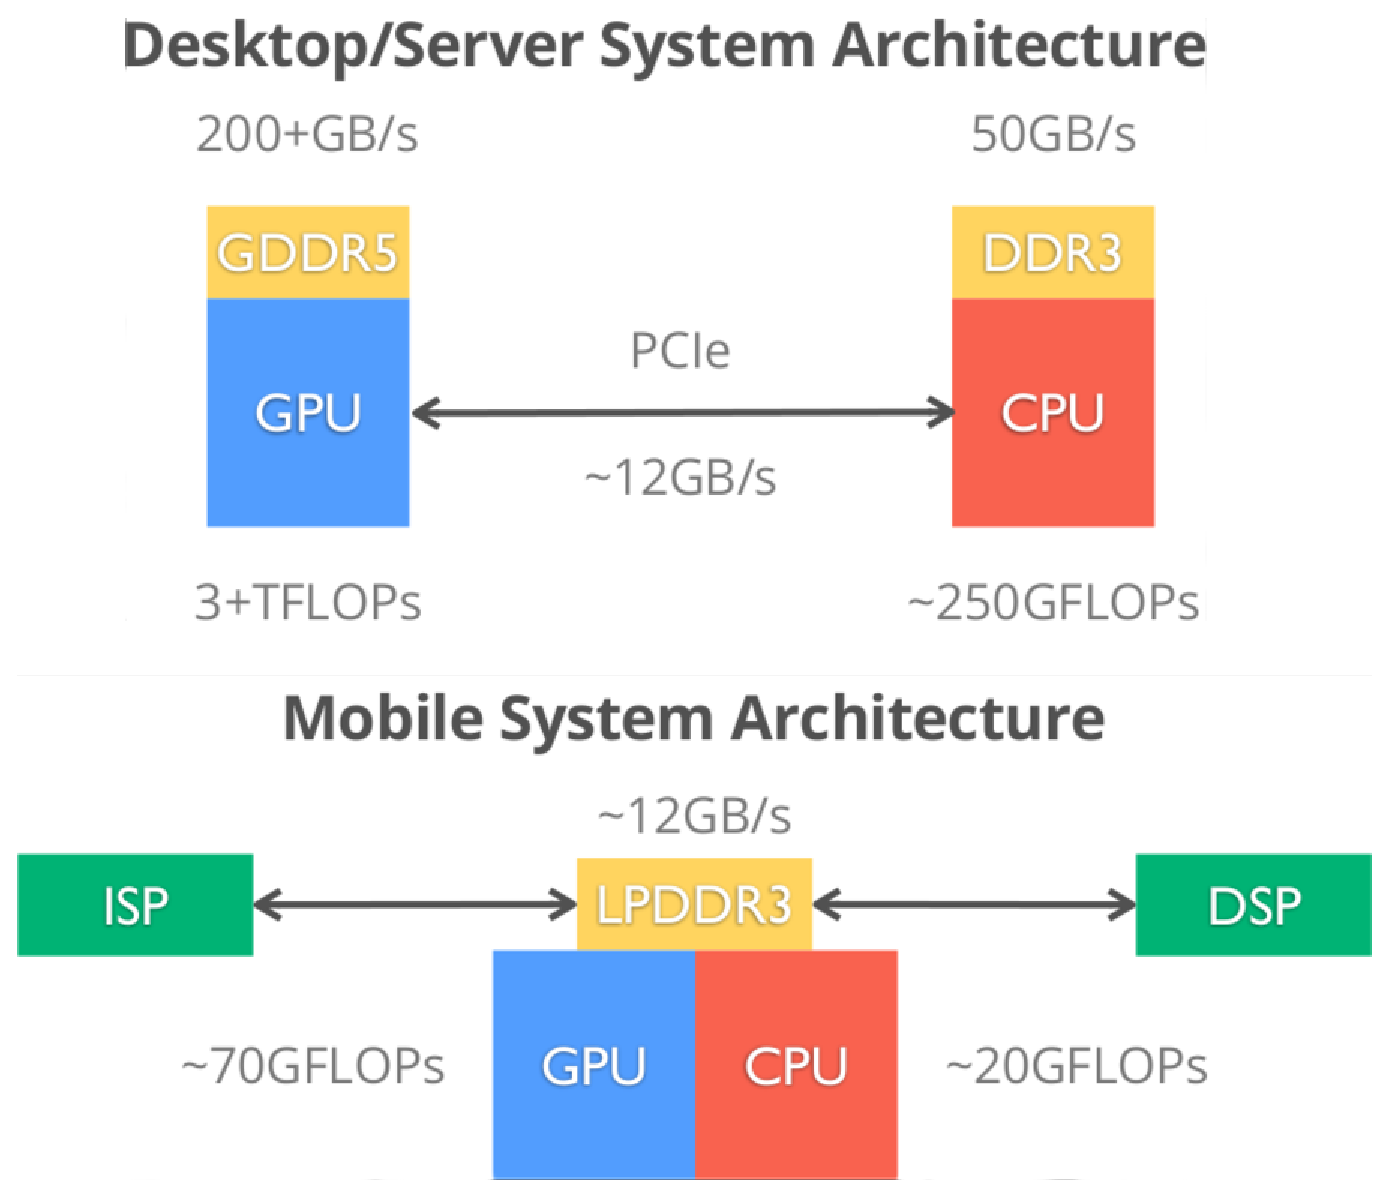
\includegraphics[width=8cm]{./pictures/desktopvsmobile}
 \caption{desktop/server architecture vs mobile architecture.}
 \label{fig:deskmob}
\end{figurehere}

\section{Why Renderscript}
The purpose of RenderScript is to develop high performance applications for a wide variety of SoCs without sacrificing portability. RS framework provides a platform-indipendent computation engine that operates at native level.

As explained in~\cite{}, we can point out three main goals, from most to least important:
\\\\
{\bf Portability}: application code should be able to run across all devices, even those with radically different hardware.

The first thing one notices about the RS API is that it is focused on the system: one doesn't get a list of devices, or a big collection of device properties so you don't have to try to figure out at run time which device you should use. The RS runtime handles that for you. You simply have a computation that you want to run quickly and the RS engine will manage to execute it on the best processor available.
\\\\
{\bf Performance}: get as much performance as possible within the costraints of portability.

RS code is firtly compiled to an intermediate and architecture-indipendent bytecode by the llvm compiler that runs as a part of an Android build. When your app runs on a device, the bytecode is compiled again just-in-time to machine code by another llvm compiler that resides on the device and optimizes the code for the particular target.
Google works with SoC vendors and gets drivers for their GPUs, DSPs, ISPs, and makes them available on tablets and phones. This way, the RS runtime knows about whatever processors and capabilities it can use.
\\\\
{\bf Usability}: simplify development as much as possible.

Java classes are reflected from RS code for an easy integration with existing applications. This allows the control of RS runtime management and execution directly through Java APIs without relying on JNI or some other low-level interface. Furthermore, a collection of RS files (called intrinsics) is provided for the standard graphic computational functions like convolution, YUV to RGB conversion and Gausian blur filtering.

\section{Writing RenderScript file}
RS files are written in a C99 derived language (C99 is the standard C from 1999, the current standard is C11, since 2011).
The main component of an RS file is a special function called kernel, here is the place where we have to write the computation we want to performe as fast as possible. Kernel functions take as input a special object called Allocation, which is nothing but a memory space with a number of elements of the same type (see {\bf Table \ref{tab:basicRS}}). The normal behavior of RS when a kernel function is called from a java application, is to launch it across all the elements inside the allocation passed by input.

Some key features of the RS runtime libraries include:
\begin{itemize}
\item Memory allocation request features.
\item A large collection of math functions with both scalar and vector typed overloaded versions of many common routines.
\item Conversion routines for primitive data types, vectors and matrix routines, date and time routines.
\item Data types and structures to support the RenderScript system such as Vector types for defining two-, three-, or four-vectors.
\item Logging functions.
\end{itemize}
See \href{http://developer.android.com/guide/topics/renderscript/reference.html}{RS runtime API reference} for more information on the available functions. \\

\begin{tablehere}
\centering
\begin{tabularx}{0.5\textwidth}{lX}
\toprule
Object & Description \\
\midrule
\textbf{Element} & An Element is essentially a C type; it can be a scalar type (e.g. an int), a vector type (e.g. an int4 or a float4) or a C struct declared on your RS code.
It represents one cell of a memory allocation. \\
\midrule
\textbf{Allocation} & An Allocation is a portion of memory containing a collection of a single type of element. It provides the memory to get data from java into RenderScript, making it processesable by one ore more kernels. \\
\midrule
\textbf{Type} & A Type is a memory allocation template and constitutes the size of the allocation. It consists of an element and one or more dimentions and describes the layout of the memory.
You can assign the X, Y, Z dimensions to any positive integer value within the constrains of available memory. So you can have a vector, a matrix or a cube of elements. That allows to do safety checking on copies and kernel launches and also to control how much parallel work actually gets launched by a kernel. \\
\bottomrule
\end{tabularx}
\caption{android object types for RS.}
\label{tab:basicRS}
\end{tablehere}

\subsection{RenderScript Kernel}
\label{sub:RSK}
An RS kernel is the portion of code that requires extensive computational horsepower and that we want to execute at high performance. It tipically resides in a \emph{.rs} file (also called script) in the \emph{project\_root/src/} directory. Each script contains is own set of kernels, variables and functions. A script can contain:
\begin{itemize}
\item A pragma declaration (\emph{\#pragma version(1)}) that declares the RenderScript version used in the script. So far 1 is the only value available.
\item A pragma declaration (\emph{\#pragma rs java\_package\_name (com.example.app)}) that indicates the package for the java classes reflected from this script.
\item Some invokable functions, i.e. single-threaded fuctions often used for initial setup.
\item A certain number of script globals equivalent to a global variable in C and almost used to pass parameters from the java side to RS kernels.
\item Some number of compute kernels, that are parallel fuctions that executes across every Element within an Allocation.
\item An optional \emph{init()} function, a special type of invokable function that runs when the script is first instantiated. This allows for some computation to occur automatically at script creation.
\item static script globals and functions. They can be used normally in any kernel or invokable function in the script, but are not exposed to the Java API. If a script global or function does not need to be called from Java code, it is highly recommended that they are declared static.
\end{itemize}

A simple kernel may look like the following:
\begin{lstlisting}[frame=single]
uchar4 __attribute__((kernel)) invert
  (uchar4 in,uint32_t x, uint32_t y) {
	uchar4 out = in;
	out.r = 255 - in.r;
	out.g = 255 - in.g;
	out.b = 255 - in.b;
	return out;
}
\end{lstlisting}
The attribute kernel applied to the function prototype denotes that is an RS kernel instead of an invokable fuction. The ``in'' argument is a special argument automatically filled in based on the input Allocation passed to the kernel launch. The returned value is automatically written to the appropiate location in the output Allocation.
A kernel may not have more than an input and an output Allocation.
A kernel may access to the coordinates of the current execution using x, y and z argument. These are optional, but the type must be uint32\_t.
\\\\
The code written in RenderScript generates reflected Java code in Android framework in order to menage the RenderScript lifetime eliminating JNI glue code. We explain this deeper in the following subsections.

\subsection{Reflected Layer}
The reflected layer is a set of classes that the Android build tools generates to allow access to the RS runtime from the Android framework. This layer also provides methods and constructors that allow you to allocate and work with memory for pointers that are defined in your RS code. The following list describes the major components reflected:
\begin{itemize}
\item Every \emph{.rs} file is generated into a class named \emph{project\_ root/gen/package\_name/ScriptC\_renderscript\_filename} of type ScriptC. This file is the \emph{.java} version of your \emph{.rs} file, which you can call from the Android framework. This class contains the following items reflected from the \emph{.rs} file:
\begin{itemize}
\item Non-static functions. Functions cannot have a return value, because the RenderScript system is designed to be asynchronous. When your Android framework code calls into RenderScript, the call is queued and executed when possible. This restriction allows the RS system to run without constant interruption and increases efficiency. If functions were allowed to have return values, the call would be blocked until the value was returned.
If you want the RS code to send a value back to the Android framework, use the \emph{rsSendToClient()} function. 
\item Non-static global RenderScript variables. Getter and Setter methods are generated for each variable so you can read and write them from Android framework. If a global variable is initialized at the RenderScript runtime layer, those values are used to initialize the corresponding values in the Android framework layer. If global variables are marked as const, then a set method is not generated.
\item Global pointers. A get method and a special method named \emph{bind\_pointer\_name} (instead of a set() method) are also generated. The second method allows you to bind the memory that is allocated in the Android VM to the RS runtime (you cannot allocate memory in your \emph{.rs} file).
\end{itemize}
\item A struct is reflected into its own class named \emph{<project\_root>/gen/package/name/ScriptField\_struct \_name}. This class represents an array of the struct, which allows you to allocate memory for one or more instances of this struct.
\end{itemize}

\subsection{Using RenderScript from java code}
Managing RS lifecycle from Android side relies on the API classes located in the \href{http://developer.android.com/reference/android/renderscript/package-summary.html}{android.renderscript}, for devices running Android 3.0 (API level 11) and higher, or in the \href{http://developer.android.com/reference/android/support/v8/renderscript/package-summary.html}{android.support.v8.renderscript} package through a Support Library, for devices running Android 2.2 (API level 8) and higher. Most applications follow the same basic usage patterns:
\begin{enumerate}
\item {\bf Initialize a RenderScript context.} The RenderScript context, created with \textit{create(Context)}, ensures that RenderScript can be used and provides an object to control the lifetime of all subsequent RenderScript objects. You should consider context creation to be a potentially long-running operation, since it may create resources on different pieces of hardware; it should not be in an application's critical path if possible. Typically, an application will have only a single RenderScript context at a time.
\item {\bf Create at least one Allocation to be passed to a script.} An Allocation is a RenderScript object that provides storage for a fixed amount of data. Kernels in scripts take Allocation objects as their input and output, and Allocation objects can be accessed in kernels using \emph{rsGetElementAt\_type()} and \emph{rsSetElementAt\_type()} when bound as script globals. Allocation objects allow arrays to be passed from Java code to RS code and vice-versa. Allocation objects are typically created using \emph{createTyped(RenderScript, Type)} or \emph{createFromBitmap(RenderScript, Bitmap)}.
\item {\bf Create whatever scripts are necessary.} There are two types of scripts available when using RenderScript:
\begin{itemize}
\item {\bf ScriptC}: These are the user-defined scripts as described in section \ref{sub:RSK} above. Every script has a Java class reflected by the RS compiler in order to make the script easy to access from Java code; this class will be named \emph{ScriptC\_filename}. For example, if the kernel above was located in \emph{invert.rs} and a RenderScript context was already located in mRS, the Java code to instantiate the script would be:
\end{itemize}
\begin{lstlisting}[frame=single]
ScriptC_invert invert =
 new ScriptC_invert(mRenderScript);
\end{lstlisting}
\begin{itemize}
\item {\bf ScriptIntrinsic}: These are built-in RenderScript kernels for common operations, such as Gaussian blur, convolution, and image blending. For more information, see the subclasses of ScriptIntrinsic.
\end{itemize}
\item {\bf Populate Allocations with data}. Except for Allocations created with android.renderscript, an Allocation will be populated with empty data when it is first created. To populate an Allocation, use one of the copy methods in Allocation.
\item {\bf Set any necessary script globals}. Globals may be set using methods in the same \emph{ScriptC\_filename} class with methods named \emph{set\_globalname}. For example, in order to set an int named elements, use the Java method \emph{set\_elements(int)}. RenderScript objects can also be set in kernels; for example, the \emph{rs\_allocation} variable named \emph{lookup} can be set with the method \emph{set\_lookup(Allocation)}.
\item {\bf Launch the appropriate kernels}. Methods to launch a given kernel will be reflected in the same \emph{ScriptC\_filename} class with methods named \emph{forEach\_kernelname()}. These launches are asynchronous, and they will be serialized following the order in which they are launched. Depending on the arguments passed to the kernel, the method will take either one or two Allocations. By default, a kernel will execute over the entire input or output Allocation; to execute over a subset of that Allocation, pass an appropriate \emph{Script.LaunchOptions} as the last argument to the \emph{forEach method}.

Invoked functions can be launched using the \emph{invoke\_function\_name} methods reflected in the same \emph{ScriptC\_filename} class.
\item {\bf Copy data out of Allocation objects}. In order to access data from an Allocation from Java code, that data must be copied back to Java buffers using one of the copy methods in Allocation. These functions will synchronize with asynchronous kernel and function launches as necessary.
\item {\bf Tear down the RenderScript context}. The RenderScript context can be destroyed with \emph{destroy()} or by allowing the RenderScript context object to be garbage collected. This will cause any further use of any object belonging to that context to throw an exception.
\end{enumerate} 

\section{Performance}
So far, there aren't many results available about the performance achievable from RenderScrit, because of the young age of the framework.
In~\cite{qian2012comparison} we can find a comparison between the three programming models in Android: Java in SDK, C++ in NDK and Renderscript. 
In order to compare them a representative application is developed in all the models, and run in an Android dual-core tablet with Honeycomb 3.2 OS.
The application chosen is \emph{Balls}, which simulate the movement of several hundred of bodies according to the gravity to the ground and repulsion among them.
{\bf Figure \ref{fig:models}} shows the best achieved performance. The device sets 60 as the maximal FPS. When the computation for one frame is faster, the device still gives 60 FPS since that is the maximal. We can see that the NDK and RS versions are quite close in performance, while the SDK version lags far behind.

\begin{figurehere}
 \centering
 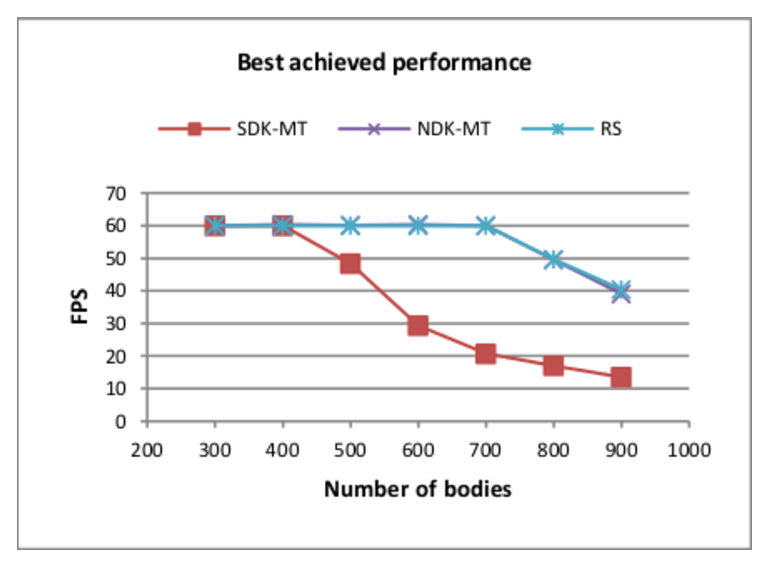
\includegraphics[width=8cm]{./pictures/models}
 \caption{best achieved performance.}
 \label{fig:models}
\end{figurehere}

However this work is quite old since in the meantime Google spent many efforts to improve performance~\cite{Rsperf:2013:Online}, especially for intrinsic kernels, as we can see in {\bf Figure \ref{fig:RSperformance}}, which shows the evolution of RS performance on Galaxy Nexus across different Android platform versions.

\begin{figurehere}
 \centering
 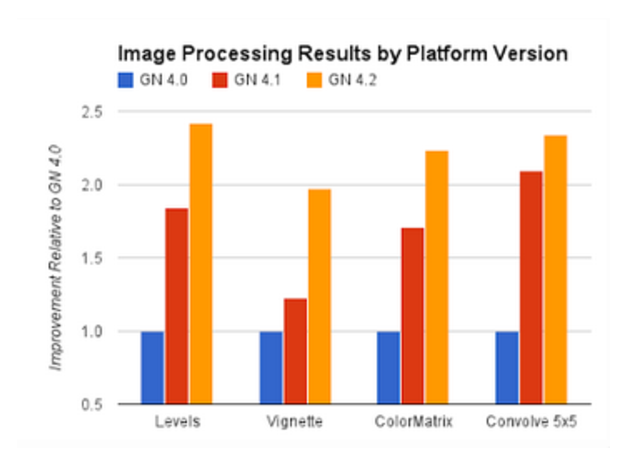
\includegraphics[width=8cm]{./pictures/perform}
 \caption{performance evolution across different Android versions.}
 \label{fig:RSperformance}
\end{figurehere}

\section{Conclusion}
RenderScript seems to be very useful when your goal is writing an application that require high-performance computational tasks in order to develop a single program that runs well on a large number of different target architectures.
In the contrary, if you mean to optimize an application for a specific target-architecture, RS is not your tool, since it decrease peak performance on specific target platform in order to guarantee very good average performace across a larger number of SoCs.
Anyway, the choice to use RS should be well pondered, since this framework brings some serious drawbacks.
First of all it increases project's complexity due to the introduction of a new set of APIs that you have to learn. While the syntax of C99 is well known, the learning curve of RS system is pretty steep, because its APIs are not. Besides the programmer must manage memory allocation manually from java layer. 
Another issue is that RenderScript can potentially execute on processors other than the main CPU (such as the GPU) and, if this occurs, debugging becomes a problem. Given the nature of RenderScript and how it works with multiple cores, this is not a huge surprise, but this can make finding and eliminating bugs more difficult.
Ultimately, the choice to use RenderScript, the NDK, or stay within the realm of Java is entirely dependent on the project's specifications. It's an application design decision with considerable ramifications, it effects what programming language you can use, what devices your application can run on, and how complicated your source project is from a maintenance perspective.

\nocite{*}
% We suggest the use of JabRef for editing your bibliography file (Report.bib)
\bibliographystyle{plain}
\bibliography{Report}

\end{multicols}

\pagestyle{empty}                  % delete footer and header

\begin{appendices}

\section{Example of an intrinsic RenderScript kernel usage}
\label{app:ex1}
\noindent Suppose we want to apply a Gaussian blur to a Bitmap image. Since Android gives an intrinsic script to implement this task we don't have to write a RenderScript file.

Here is the auto-esplicative code to use on Java side in order to correctly utilize Android API.

\begin{lstlisting}[frame=single]

// Create a Context
RenderScript mRS = RenderScript.create(this);

// Create a RenderScript Allocation to hold the input image.
Allocation inputAllocation = Allocation.createFromBitmap(mRS, myInputBitmap,
	Allocation.MipmapControl.MIPMAP_NONE,
	Allocation.USAGE_SHARED |
	Allocation.USAGE_GRAPHICS_TEXTURE |
	Allocation.USAGE_SCRIPT);

// Create an output Allocation, notice the USAGE flags are different
Allocation outputAllocation = Allocation.createFromBitmap(mRS, myOutputBitmap,
	Allocation.MipmapControl.MIPMAP_NONE,
	Allocation.USAGE_SHARED |
	Allocation.USAGE_SCRIPT);

// RenderScript has built in support for Blur so use that
ScriptIntrinsicBlur mBlur;

// First, we need to create the intrinsic
mBlur = ScriptIntrinsicBlur.create(mRS, Element.U8_4(mRS));

// And now we configure the intrinsic to perform our blur
mBlur.setRadius(20.f);
mBlur.setInput(inputAllocation);

// Now run the blur
mBlur.forEach(outputAllocation);

// Copy the output to our bitmap if necessary
outputAllocation.copyTo(myOutputBitmap);


\end{lstlisting}
\vspace{4ex}
And this is our image before and after the filter application:

\begin{figurehere}
 \centering
 
\includegraphics[width=0.5\textwidth]{./pictures/childhood}
 \label{fig:childhood}
\end{figurehere}
\begin{figurehere}
 \centering
 
\includegraphics[width=0.5\textwidth]{./pictures/childhoodblur}
 \label{fig:childhoodblur}
\end{figurehere}


\section{Example of a RenderScript kernel writing and usage}
\label{app:ex2}
\noindent In this example we compute the luminance histogram of an image, but we want to do it in two separate steps:
\begin{itemize}
\item in the first step the image is splitted in stripes and for each one the histogram is computed.
\item the second step sums the histograms obtained from the previously step.
\end{itemize}
For implementing the program in the way described above we need to write two different kernel functions.
\\\\
This is the code for the RenderScript runtime framework, which resides in our .rs file:

\begin{lstlisting}[frame=single]

// The histogram script requires a number of buffers

// The source and destination images.
rs_allocation gSrc;
rs_allocation gDest;

// A buffer for the intermediate sums
// Integer values, [256][steps] in size
rs_allocation gSums;

// Final sum buffer, Integer, [256] cells in size
rs_allocation gSum;

// The height and width of the image
int gWidth;
int gHeight;

// The step, which is the number of lines processed by each thread
int gStep;

// The number of steps in total, roughly height / step
int gSteps;

// The start of the first kernel
void __attribute__((kernel)) pass1(int in, uint x, uint y) {
  // Note that x and y will indicate the coordinates of the pixel being processed
  // This kernel will be run on a range of x = [0] and y = [0 to steps]
  // Clear our output buffer for this thread.
  for (int i=0; i < 256; i++) {
    // Set the value at i,y to 0
    rsSetElementAt_int(gSums, 0, i, y);

  }

  // Iterate over our image
  for (int i= 0; i < gStep; i++) {
    int py= y*gStep + i;	// Compute the y coordinate in the image
    if (py>= gHeight) return;	// Might be out of range if this is the last step

    // Walk one scanline
    for (int px=0; px < gWidth; px++) {
      // Get the pixel and convert to luminance
      uchar4 c = rsGetElementAt_uchar4(gSrc, px, py);
      int lum = (77 * c.r + 150 * c.g + 29 * c.b) >> 8;

      // Add one to the bucked for this luminance value
      int old = rsGetElementAt_int(gSums, lum, y);
      rsSetElementAt_int(gSums, old+1, lum, y);
    }
  }
}

// This kernel is run on the Sum allocation, so its called once
// for each of the 256 levels
// Note, this is a 1D kernel
int __attribute__((kernel)) pass2(uint x) {
  int sum = 0;

  // For this level, add in the sum from each of the
  // separate partial sums
  for (int i=0; i < gSteps; i++) {
    sum += rsGetElementAt_int(gSums, x, i);
  }

  // Return the sum for this level. Since this is a kernel
  // return value, it will automatically be placed in the allocation.
  return sum;
}

// This is an invokable function. It will be called single threaded
void rescale() {
  // Find our largest bucket value
  int maxv = 0;
  for (int i=0; i < 256; i++) {
    maxv = max(maxv, rsGetElementAt_int(gSum, i));
  }

  // Compute the rescale value to to convert bucket values into bar heights.
  float overMax = (1.f / maxv) * gHeight;

  for (int i=0; i < 256; i++) {
    int t = rsGetElementAt_int(gSum, i);
    t = gHeight - (overMax * rsGetElementAt_int(gSum, i));
    t = max(0, t);
    rsSetElementAt_int(gSum, t, i);
  }
}


\end{lstlisting}

\vspace{4ex}
This is the code we have to write in the Java application that allows to launch our scripts:

\begin{lstlisting}[frame=single]

// Create and load the script
mScript = new ScriptC_histogram(mRS);

// Setup the globals
mScript.set_gWidth(width);
...

// Create the [256][steps] buffer of integers for the partial sums
Type.Builder tb = new Type.Builder(mRS, Element.I32(mRS));
tb.setX(256).setY(steps);
Type t = tb.create();
mSums = Allocation.createTyped(mRS, t);

// Create the 1D [256] buffer for the final Sums
mSum = Allocation.createSized(mRS, Element.I32(mRS), 256);

// Set the buffers for the script
mScript.set_gSums(mSums);

// This first pass should be clipped because we want [step] threads
// not [256][step] threads

// To do this we have the ability to clip our launch
// using a LaunchOptions class
Script.LaunchOptions lo = new Script.LaunchOptions();

// Set the range in the X dimension to be 0 to 1
// Note: the end is exclusive so this says only run X value 0
lo.setX(0, 1);

// Run the kernel with our launch options
// This will spawn one thread per Y coordinate, each with X=0
mScript.forEach_pass1(mSums, lo);

// Once the first pass is complete, we need to add up our partial sums

// The pass2 launch is unclipped.
// It spawns one thread per cell in the mSum buffer
// for a total of 256 threads.
mScript.forEach_pass2(mSum);

// Finally, we call our rescale function
mScript.invoke_rescale();


\end{lstlisting}
\vspace{4ex}
This is an example of an image with its luminance histogram:

\begin{figurehere}
 \centering
 
\includegraphics[width=0.5\textwidth]{./pictures/bitmap}
 \label{fig:bitmap}
\end{figurehere}
\begin{figurehere}
 \centering
 
\includegraphics[width=0.5\textwidth]{./pictures/lumhist}
 \label{fig:lumhist}
\end{figurehere}


\end{appendices}
\end{document}

